\chapter{FPV車両操作の体感速度変化率の定式化}
\section{はじめに}
体感速度の変化とは、基準となる速度に対して、観測環境における何らかのパラメータの作用により、視覚的な体感情報から得られる速度感覚が基準と比べて変化する現象のことである。
自動車を運転する際、車速の増加によってドライバの有効視野角が狭まり、ドライバの体感速度が減少する現象が報告されている。
また、低速状態においても、ドライバの視野角の変化、運転視野映像のクロップによって体感速度が変化する現象が一般的に知られている。
また、自動車等を、カメラ映像を確認しながら遠隔操作(FPV:First Person View操作)する際に、カメラの設定によって同様の現象が起こる。
これはカメラ映像による視覚情報が、遠隔操作を行うための操作者への体感情報に影響を与えるためだと考えられている。
具体的には、カメラの画角の設定などが挙げられる。FPVは、操作対象から見た視点であり、操作者が操作対象から周囲の景色を見ることを目的としている。
自動車の運転操作と、遠隔型自動運転や、FPVによるRCカーの操作では、スケールの違いや、カメラの画角の設定等から、視覚情報から得られる体感情報において矛盾が生じる。
一例として、操作対象自身の視点から体感する感覚的な移動速度(体感速度)を錯覚する。
一般に、自動車のドライバが利用する情報のおよそ 90\%が 視覚情報であると報告されており、ドライバが受け取る情報の大部分を占めているため、体感速度の錯覚が、適切な運転に影響を与え、思わぬ事故を引き起こす恐れがある。
体感速度の錯覚は、走行環境と自動車の運転速度の変化によっても生じる。より広い道路を高速で移動すると、人間の視野における周辺視の減少により、自動車の体感速度を実際の速度よりも低く感じるように錯覚すると報告されている。
高速道路等で体感速度を低く感じると、ドライバは、車速を増加させる傾向にある。車速の増加が自動者事故の原因になる。
また、逆に低速域においても視野角の減少によって体感速度が減少することが報告されている。また、ゲーム等の演出で使用されているものとしては、視野を広げると速く見せることができる。
一方、運転映像や運転中の視野角の変化による体感速度の比率の定量化に関しては行われていない。視野角を狭めることによる効果や、視野の増加によって得られる体感速度の定量化\verb|(モデル化)|はされていない。
また、視野角の減少と増加の両方における体感速度の変化を一つの特性として表した例はない。
体感速度を定式化することができれば、映像から得られる視覚効果の影響を光学的に応用し、FPV操作や、ヘッドアップディスプレイ等によって、ドライバの体感情報の補正手法としての応用が期待できる。
そこで我々は、自動車の映像における体感速度のモデルの定量化を目的として、体感速度モデルの定式化を提案する。
DSの走行映像において観測者の体感速度の減少を促す映像クロップと視野角の特性を求め、クロップ率-体感速度と、視野角-体感速度の幾何学モデルを定式化する。
本研究では、クロップ率・視野角の減少と増加の特性を一つのモデルとして表し、視野角の変化に対する体感速度の変化を定式化することで、映像から得られる体感速度を定量的に定義した。

\section{従来研究}
淺田ら\cite{taikan:asada}は、人間の視覚情報を用いた体感速度変化を利用した研究として、ドライビングシミュレータの操作視点にバーチャルパターンを投影することによって、ドライバに適切な速度制御を促す手法が提案されている。
運転者の速度制御をモデル化することにより、ドライバが適切な速度を制御できない要因として「環境からの速度認知に関する誤差が大きいこと」、「目標速度設定が適切でないこと」の2点が挙げられることを明らかにした。
前者の要因を改善するバーチャルパターンとして、一定速度で移動するバーチャルパターン、流れる風景を誇張表現するバーチャルパターンを挙げ、バーチャルパターン投影映像の視聴実験の被験者の主観評価により、これらの有効性を確認した。
これらは、目標速度制御のための定性的な効果であり、体感速度の変化に寄与するパラメータについては言及されておらず、体感速度の変化を示すものは、被験者の主観による評価であるため、視覚効果の定量的な評価はされていない。

大前ら\cite{taikan:ohmae}は、遠隔操縦に基づく資格情報の影響を評価し、遠隔操縦において、カメラ条件や映像条件が運転操作に与える影響を評価している。評価結果に基づいて遠隔操縦車両および、その制御系を構築し、遠隔操縦と直接運転を比較することで、本研究で構築した遠隔操縦システムの構成により、直接運転と近い運転操作が実現できることを明らかにした。
視覚情報の影響評価においては、カメラの視野角の影響が大きく、フレームレートや解像度などの影響が相対的に小さいことが報告されている。
以上より、遠隔操縦における視覚情報の運転への影響として、視野角による影響が大きいことが述べられている。

Speed Management \cite{taikan:speedmanagement}によると、速度が上がるとドライバの視野が狭くなることが報告されている。
時速40 km の場合、ドライバの視野は 100度であり、路傍の障害物やその他の潜在的な危険を確認できる。図\ref{taikan:speed}に視野角と体感速度の関係を示す。
時速 130 km では、視野は約 30°にまで減少し、ドライバが潜在的な危険を判断する能力が大幅に低下するとされている。

\begin{figure}[h]
  \begin{center}
  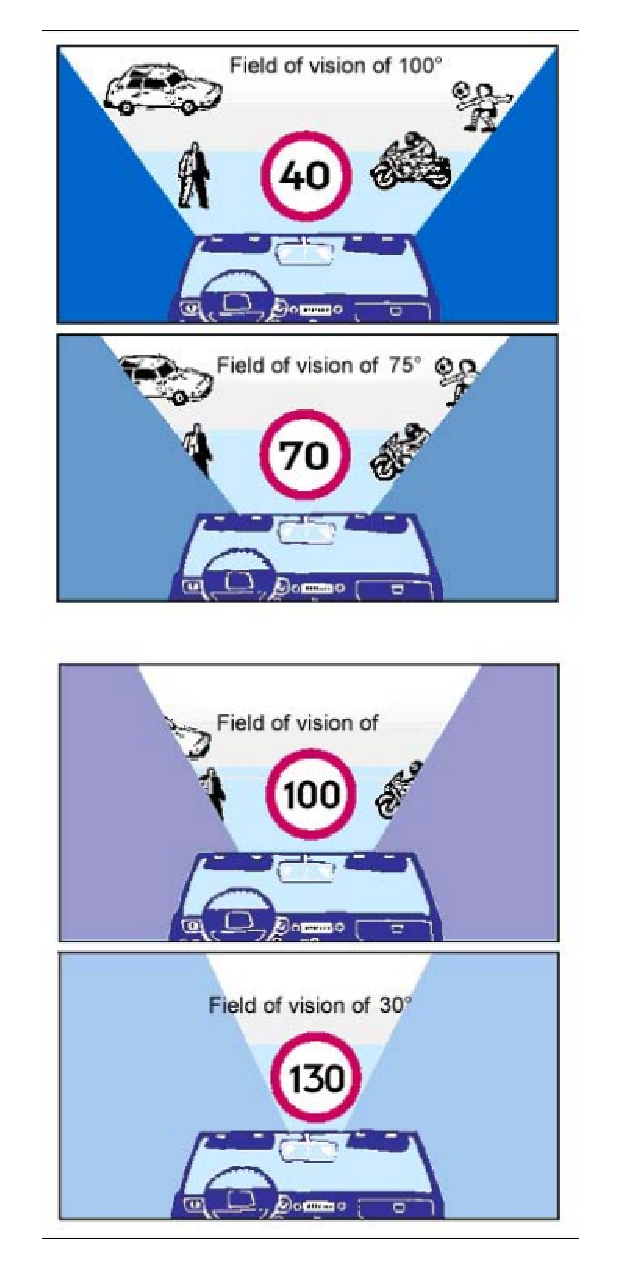
\includegraphics[width=.5\linewidth]{img/1.eps}
  \caption{視野角と体感速度の関係\cite{taikan:speedmanagement}}
  \label{taikan:speed}
  \end{center}
\end{figure}

\clearpage
体感速度を支配するパラメータとして、運転者の速度に影響を与えるパラメータに関する研究をいくつか述べる。

AR 技術を用いて運転者の体感速度を変化させる試みとして東井ら\cite{taikan:higashii}は単純な線や四角形からなるパターン の速度を実際よりも速く表示することで運転者の体感速度を変化させることに成功していた。しかし、実際にどのような速度制御が行われるかや他の表示方法で表示した場合の効果は未知数である。

走行速度と道路環境の関係についての調査として Gitelman\cite{taikan:gitelman}らは運転者が速度超過する原因は道路環境から人々が適切と感じる速度と制限速度があっていないこととし, どういった要素が適切と感じる速度に影響を与えているかを実際の道路環境の要素の調査と運転者への意識調査によって検証した。結果として視野的狭窄や歩行者の活動、道路のレイアウト等が要素として挙げられることが分かった。

Joら\cite{taikan:jo}は、運転速度がドライバの視覚的注意に及ぼす影響を、ドライバが処理できる視覚情報の最大量とのバランスがとれる最大視野という観点から評価を行った。
運転速度の増加により、処理する視覚情報の量が増加するため、ドライバが処理する視覚情報の量が、自身の取得できる最大量と釣り合う点までしか視野を広げることができないとした。
この点を超えるとドライバは、不安、ストレスの増加によりドライバが取得できる最大の視覚情報が減少し、視野がさらに狭くなって心理的圧迫感を感じる現象(トンネル効果)が起きる可能性があると述べている。具体的に、ドライバは、潜在的な危険があった場合に対処するための時間を確保するために、運転速度が上がるにつれて遠くを見る傾向がある。 これは、運転速度の増加による流体刺激の増加だけでなく、遠くを見ることでの視野の増加により、ドライバが処理する視覚情報の量が増加し、ドライバの精神的負担が増大することを意味する。ドライバは、安全を確保するために、取り扱える視覚情報の量が許される限り、可能な限り多くの視覚情報を取得する傾向にある。しかしながら、前述したように、運転者が取り込める最大の視覚情報は、運転の専門知識のレベルに応じて個人差がある。走行速度が取り込める視覚情報の許容量が釣り合う点を超えた場合、ドライバは自動的に視野を狭めることで視覚的情報の許容が釣り合う点を自己維持しようとし、処理する視覚情報の量を減らす。
一部のドライバにとっては、バランス点を超える不安ストレスが非常に高くなり、バランス点を超えた後に処理できる最大の視覚情報がさらに減少するとしている。

\section{体感速度のパラメータの模索}
RCカーと実車の速度が視覚的に一致すること(体感速度が一致すること)を目的として、体感速度の変化を及ぼすパラメータを、RCカー・DSの走行映像の比較により調査した。体感速度の比較について、車両模型の迫力・臨場感の表現として用いられるスケールスピードとの比較も行った。これにより体感速度の一致の目標が、走行映像中における単位時間当たりの描画の移動ピクセル数の一致であることが分かった。また、この目標を達成するためのパラメータを明らかにした。

\subsection{原理}
図\ref{taikan:genri}に、体感速度の原理を示す。
一般に、トラックなど乗用車よりも車高が高くなる車両を運転する場合、体感速度は遅くなり、
逆に、レースカート等の車高の低い車両を運転すると体感速度は速く感じる。RCカーを運転する場合は後者に相当する。その原理を幾何学的に説明する。

\begin{figure}[h]
  \begin{center}
  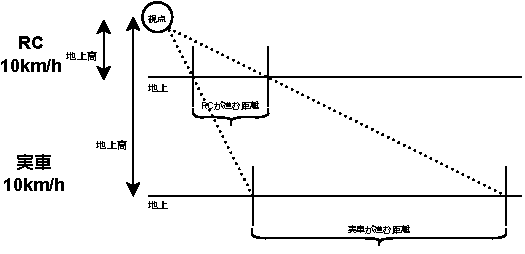
\includegraphics[width=.95\linewidth]{img/2.pdf}
  \caption{体感速度の原理}
  \label{taikan:genri}
  \end{center}
\end{figure}

体感速度の変化は上下・左右方向の視野それぞれの影響が存在する。
一例として上下方向の視野の場合を説明する。操作視点が高い時の視点は、低い時の視点の延長線上にある。
ある点から他方の点まで進んだ時も同様になる。実車あるいはRCカーが、体感的と同じ速度で移動しているための条件は、画面上のピクセルの移動速度(実際の線を移動する時間)が、実車とRCカーで同じになることである。
RCカーと実車で速度が同じでも、風景が移動する速度が異なるために体感速度が異なる。
このRCカーの実速度に対して体感速度が同じになる実車の速度との比を求めることで、体感速度の一致を求めることができる。
つまり、体感速度の一致を走行映像中の単位時間当たりの移動ピクセル数の一致とする。

\subsubsection{体感速度とスケールスピードについて}
スケールスピードとは、模型車両の実際の移動速度にスケール比の平方根を乗じたものを、実際の車両のスケールでの速度としたものである。
実際の速度にスケール比を乗ずるのではなく、力学的な相似効果から迫力の表現として使用されている。
スケールスピードの導出には、流体分野における流れの相似の指標とするフルード数が用いられ、以下のようにして導出する。

フルード数$Fr$の定義は、式\eqref{taikan:eq:frude}で表される。

\begin{align}
  Fr = \frac{U}{\sqrt{Lg}} \label{taikan:eq:frude}
\end{align}

ここで、$U$:体感速度\si{[m/s]}、$L$:代表長さ\si{[m]}、$g$:重力加速度\si{[m/s^2]}である。実車の特性速度、代表長さをそれぞれ、
$U_1$、$L_1$、RCカーの特性速度、代表長さを$U_2$、$L_2$とすると、それぞれが力学的に相似であることから、フルード数が一致するという条件のもとで、
立式すると式\eqref{taikan:eq:frude2}、\eqref{taikan:eq:frude3}のようになる。

\begin{align}
  \frac{U_1}{\sqrt{L_1g}} = \frac{U_2}{\sqrt{L_2g}} \label{taikan:eq:frude2}\\
  U_2 = \frac{U_1}{\sqrt{\frac{L_1}{L_2}}} \label{taikan:eq:frude3}
\end{align}

$\frac{L_1}{L_2}$は、実車とRCカーのスケール比であるため、特性速度、$U_2$がRCカーのスケールスピードであり、実車の速度$U_1$をスケール比の平方根で除すると求めることができる。

\subsection{DS・RCカーの走行映像の解析}
ここでは、DSとRCカーの走行映像の比較について述べる。
DS上の実速度とRCカーのスケールスピードが一致する場合RCカーと実車の体感速度が等しいと仮定して、
RCカーとDSの走行映像の単位時間あたりの移動ピクセル数の一致を目指す。またスケールスピードではなく、スケール比を乗じた速度での走行映像との比較も行った。

\subsubsection{実験方法}
\begin{enumerate}
  \item RCカーの走行環境を作成する。図\ref{taikan:rc}に、RCカーの走行環境を示す。今回は移動ピクセル数の比較のために、コース車両の脚部分に黄色い装飾を施した。RCカーに設置したカメラで定速走行映像を撮影し、始点・終点間の動画の再生時間で除して実速度を求め、スケール比の平方根との積によりスケールスピードを計算する。RCカーの移動速度は、RCカーのDCモータのPWM制御によって行われているため、PWM周期の入力値と出力値を実測する。この出力値を用いてRCカーの移動速度を計算している。
  \item DS上で実車スケールのRCカーの走行環境を作成する。図\ref{taikan:ds}にDS上で再現したRCカーの走行環境を示す。RCカーの現物の環境と視覚的な条件を等しくするために、RCカーの走行実験で使用した環境の壁面\verb|(机)|の寸法を測定し、走行路面をテクスチャマッピングによって再現した。
  \begin{figure}[h]
    \begin{center}
    \subfigure[RCカーの走行環境]{
    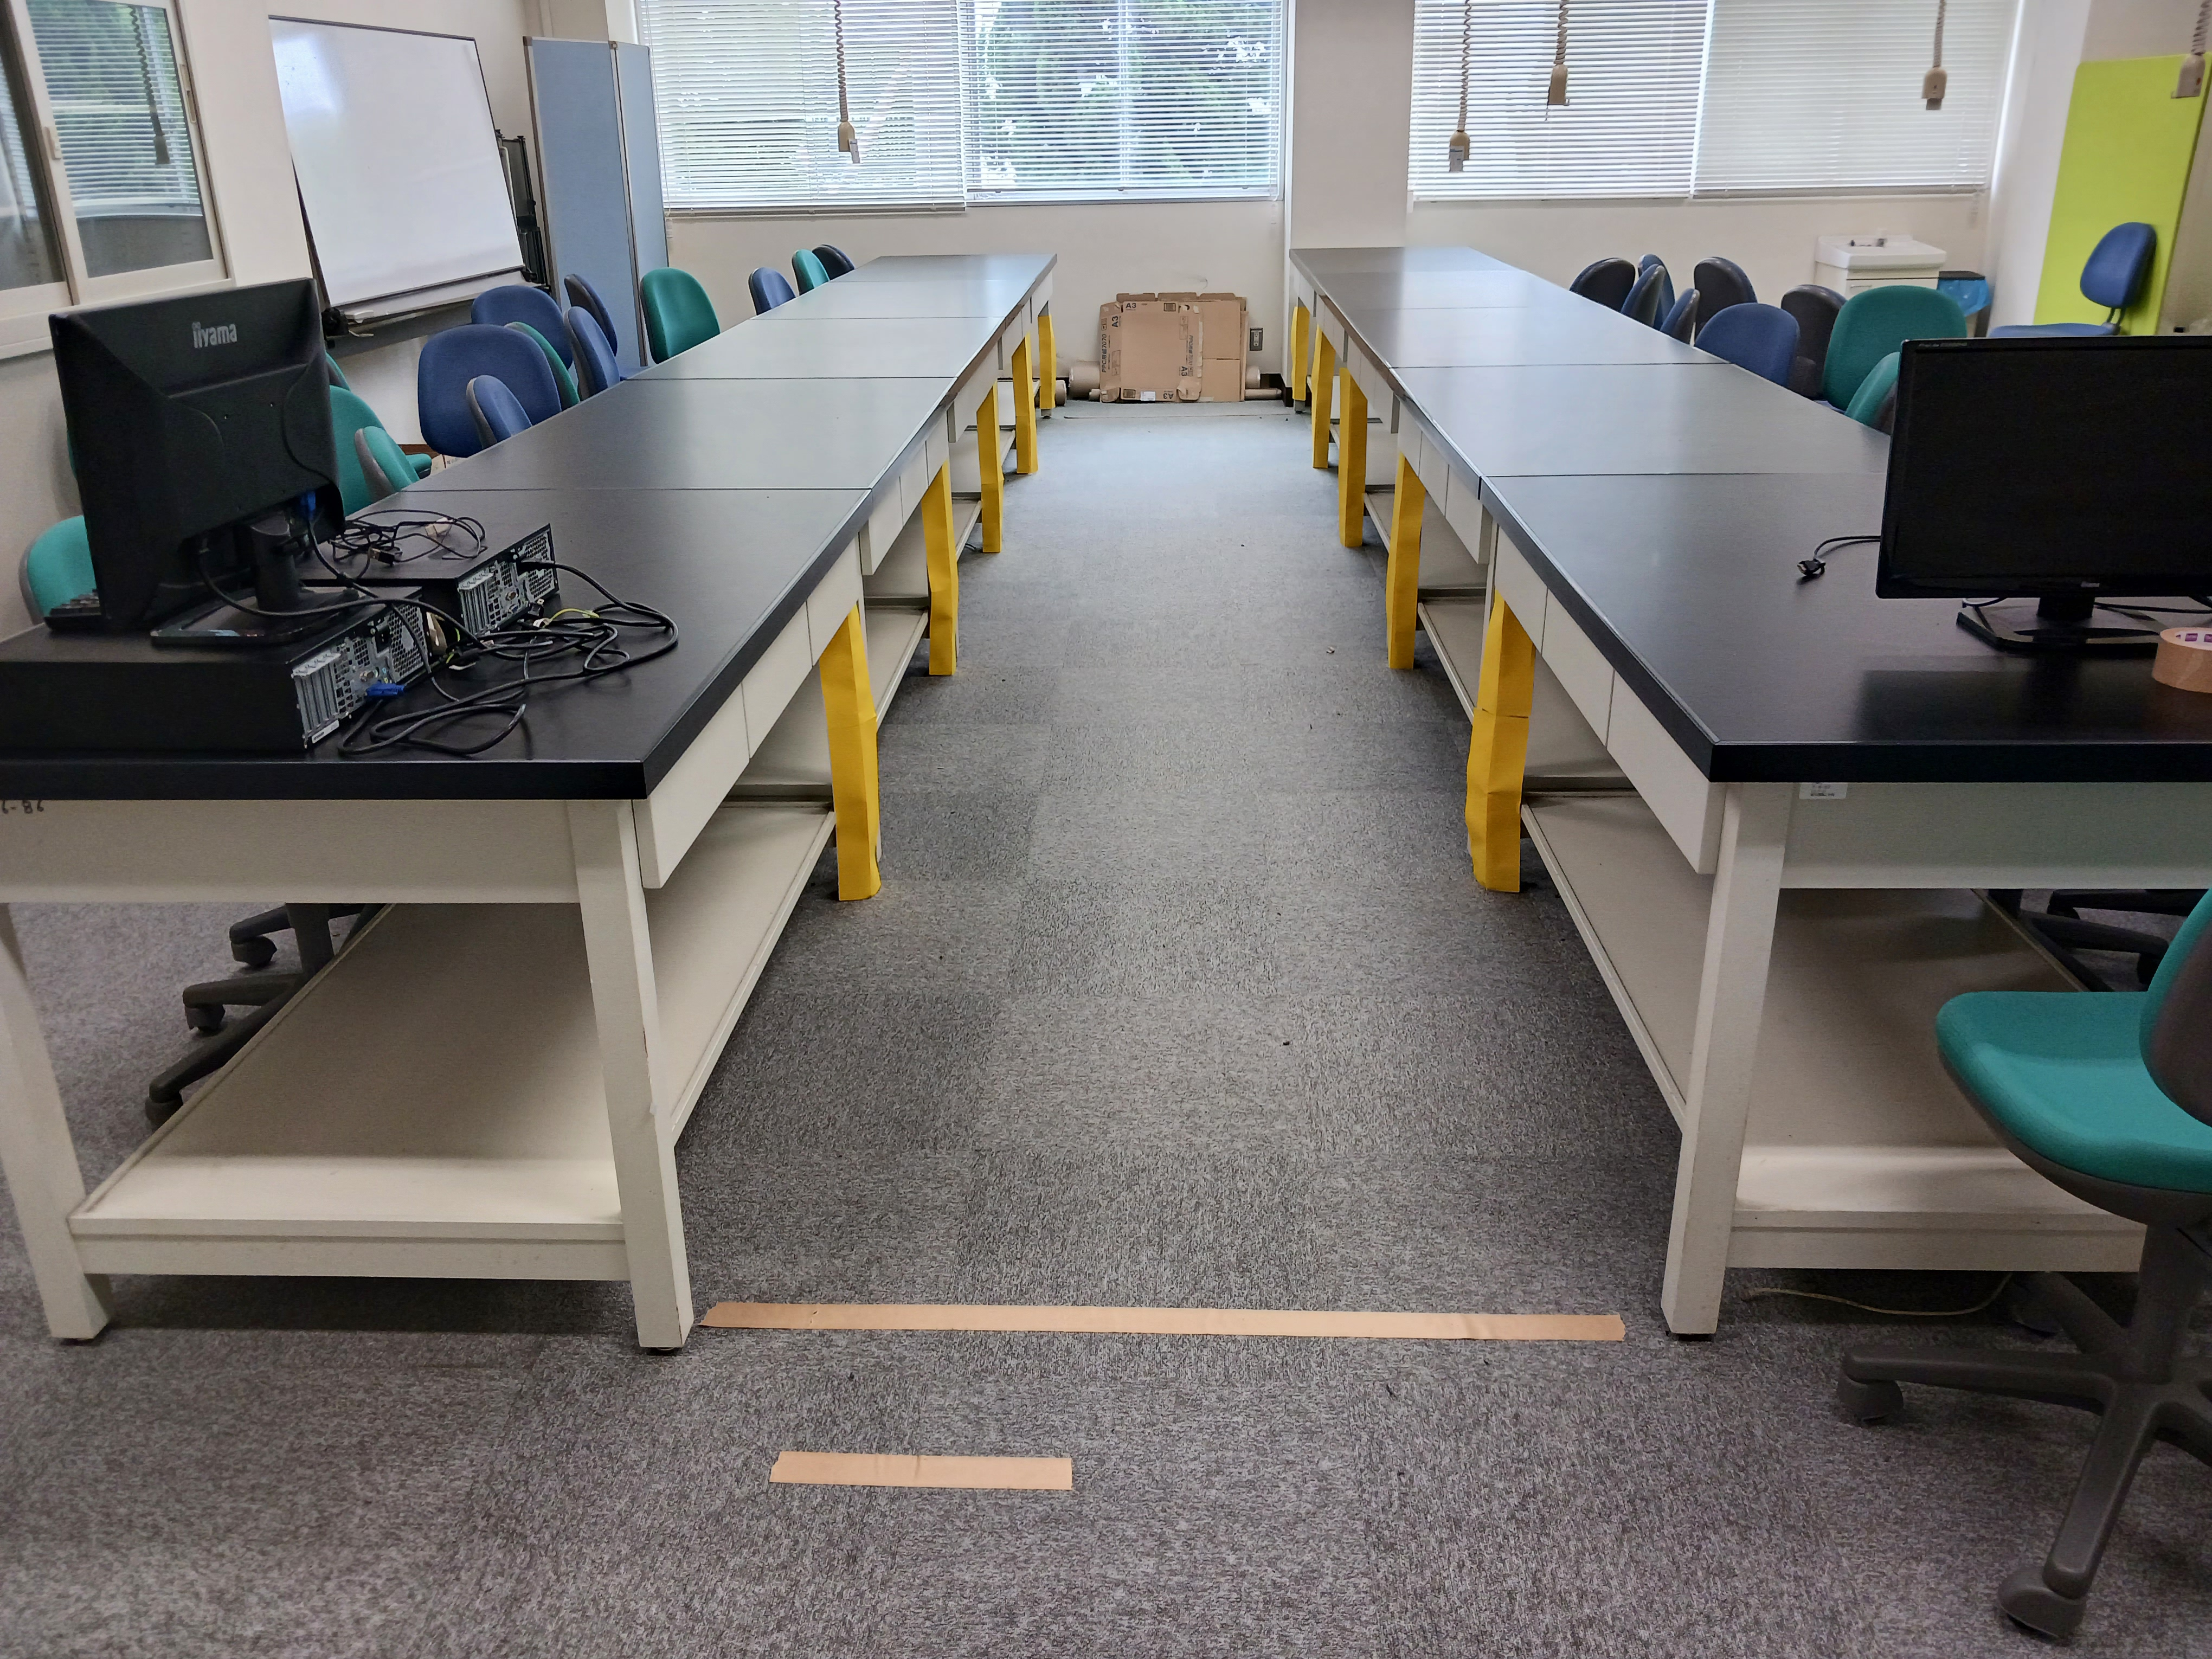
\includegraphics[width=.4\columnwidth]{img/3.jpg}
    \label{taikan:rc}
    }
    \subfigure[DS上で再現したRCカーの走行環境]{
    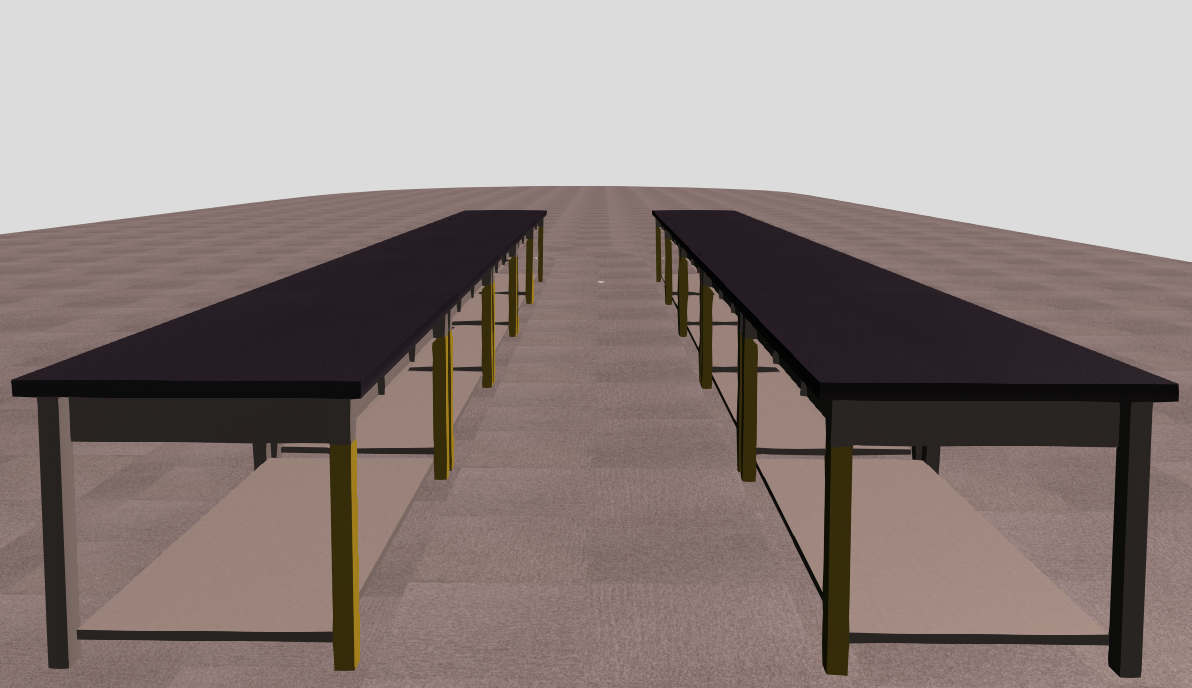
\includegraphics[width=.52\columnwidth]{img/4.png}
    \label{taikan:ds}
    }
    \caption{体感速度の実験環境}
    \label{taikan:jikken1}
    \end{center}
  \end{figure}
  \item DSの走行環境においてRCカーのスケールスピードで走行した映像を撮影する。DSとRCカーの走行映像を見比べて、単位時間当たりに通過するポールの数を目視で確認し、スケールスピードと体感速度の一致・不一致を評価する。
  \begin{figure}[h]
    \begin{center}
    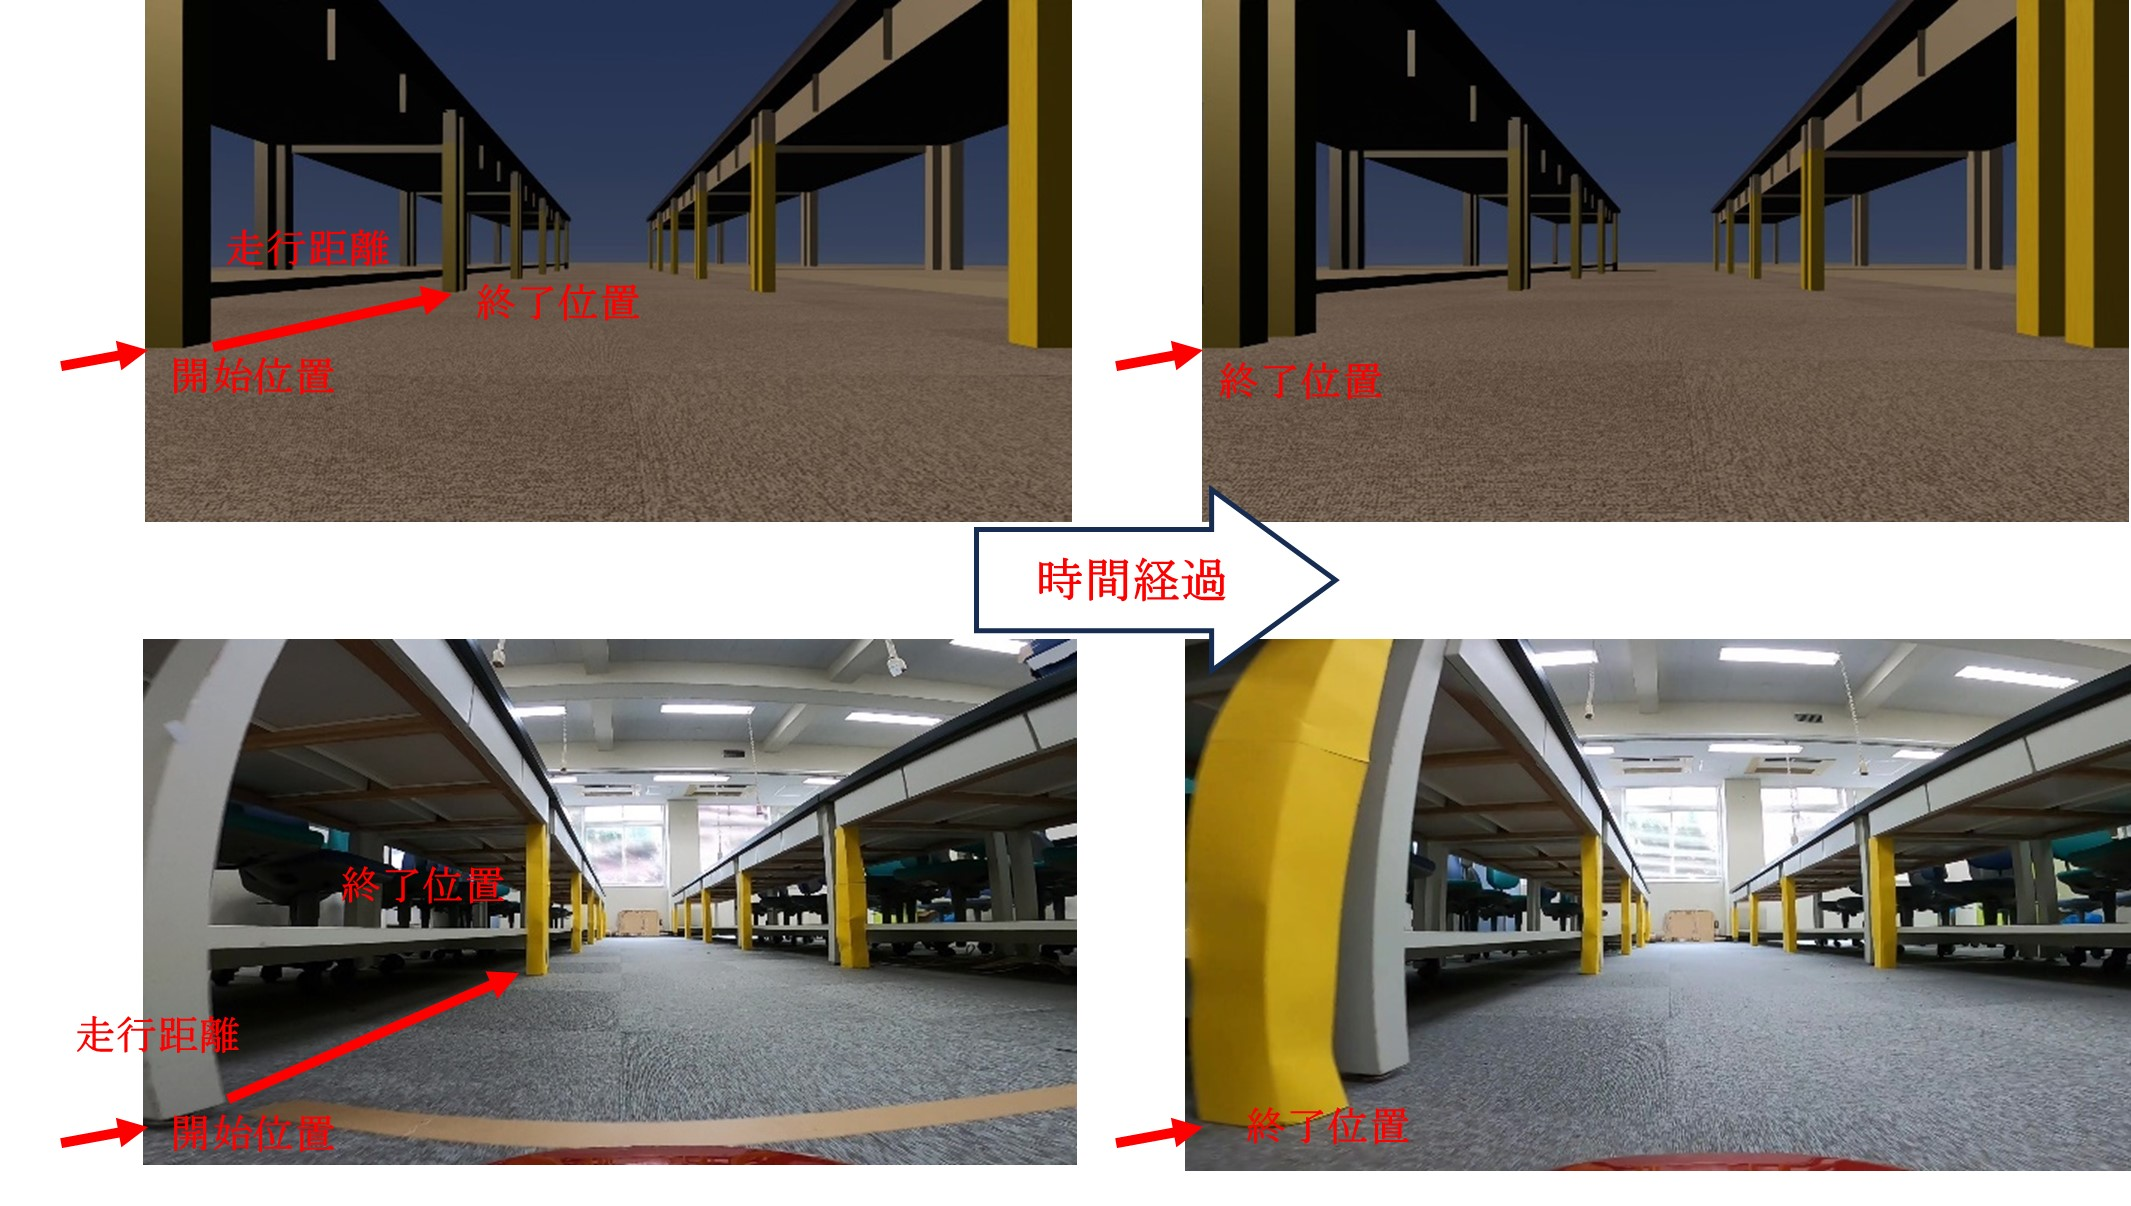
\includegraphics[width=.88\linewidth]{img/5.jpg}
    \caption{単位時間当たりに通過するポールの数の確認}
    \label{taikan:pall}
    \end{center}
  \end{figure}
  \item RC映像にスケール比を乗じた速度のRCカーの走行映像を取得する。
  \item スケールスピードでの比較とスケール比をかけた速度を比較する。
  \item 体感速度が一致しない場合、その原因を検討し、パラメータとする。
\end{enumerate}
なお、本実験で作成したDS環境の寸法を図\ref{taikan:dsm1}、\ref{taikan:dsm2}に示す。DS上の環境に関しては、RCカーのスケール比に合わせて作成した。
今回用いたRCカーのスケールが$\frac{1}{10}$であったため、実際のRCカーの走行環境を10倍したDS上の走行環境とした。

\begin{figure}[h]
  \begin{center}
  \subfigure[DS上コースの寸法:全体]{
  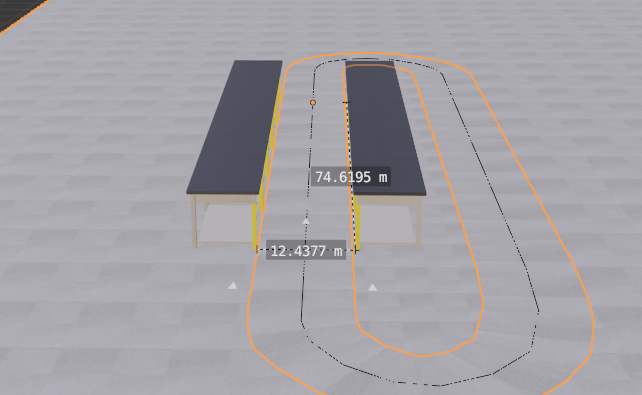
\includegraphics[width=.8\columnwidth]{img/6.png}
  \label{taikan:dsm1_1}
  }
  \subfigure[DS上コースの寸法:全長]{
  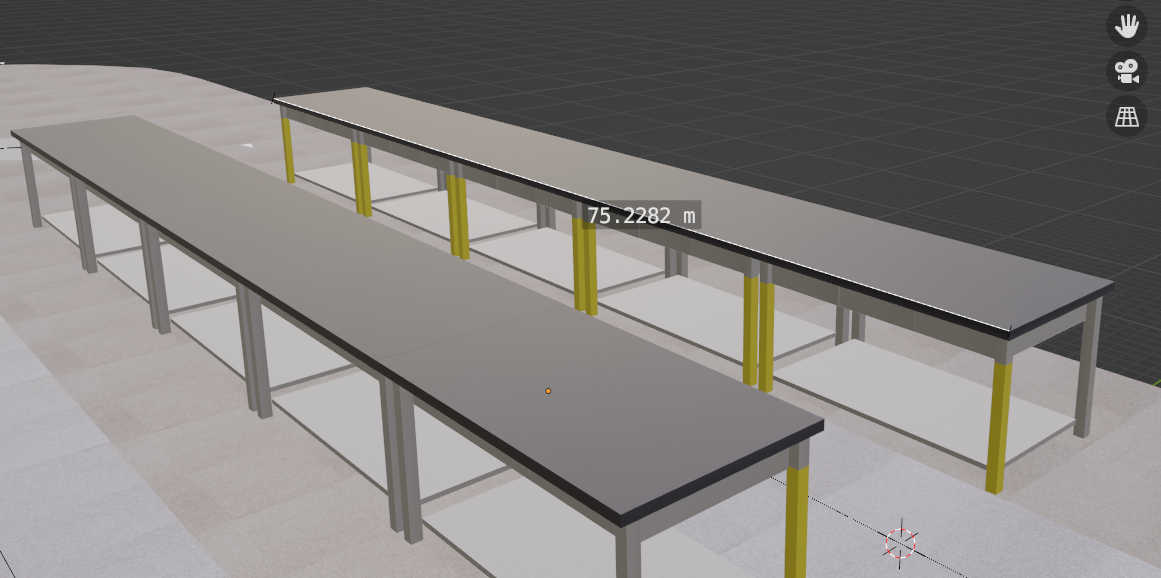
\includegraphics[width=.8\columnwidth]{img/7.png}
  \label{taikan:dsm1_2}
  }
  \caption{DS環境の寸法:全体}
  \label{taikan:dsm1}
  \end{center}
\end{figure}

\begin{figure}[h]
  \begin{center}
  \subfigure[DS上コースの寸法:障害物]{
  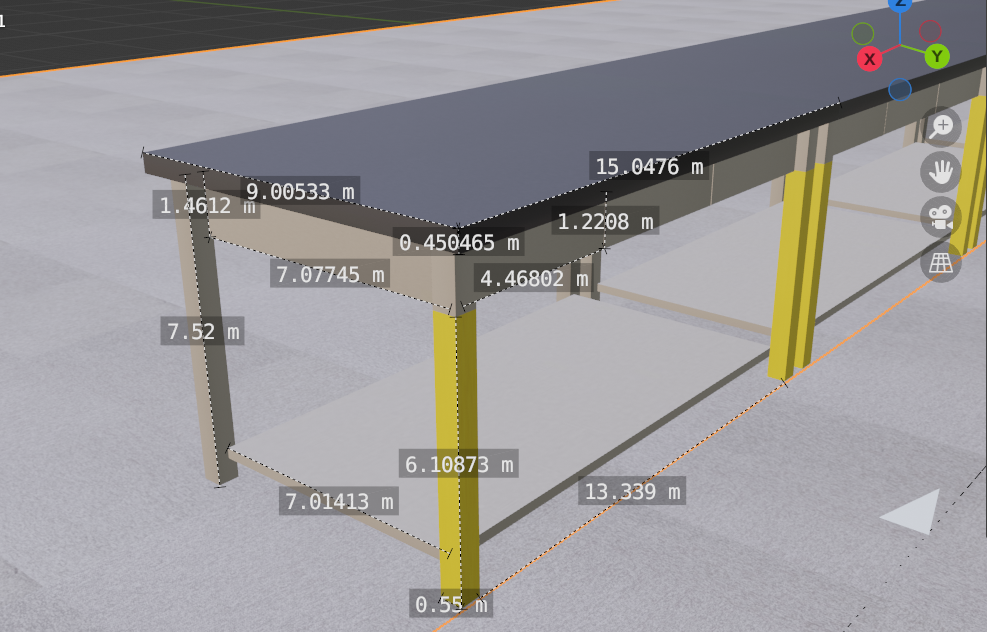
\includegraphics[width=.8\columnwidth]{img/8.png}
  \label{taikan:dsm2_1}
  }
  \subfigure[DS上コースの寸法:道幅]{
  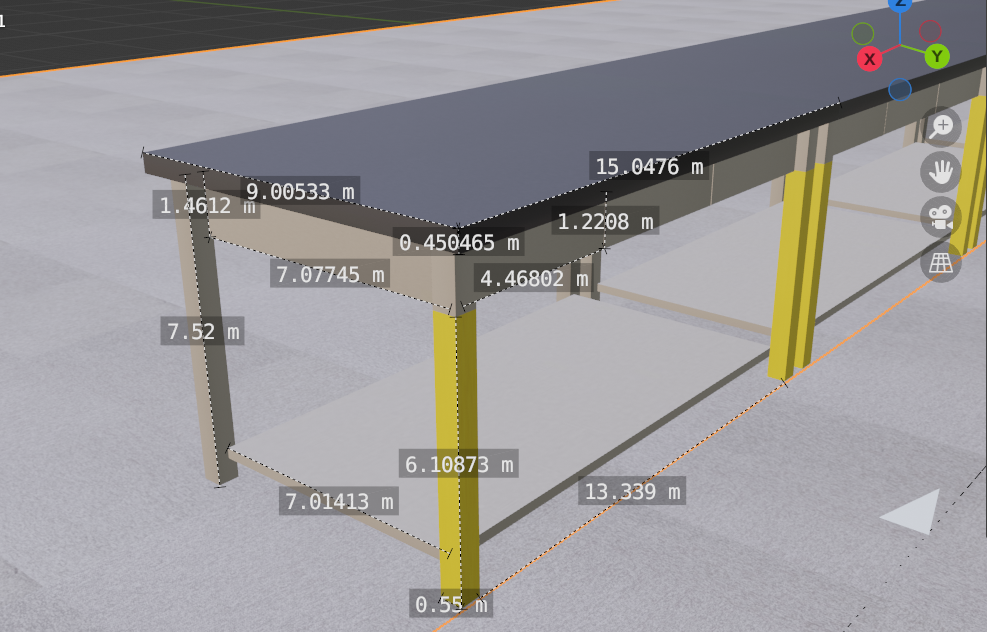
\includegraphics[width=.8\columnwidth]{img/8.png}
  \label{taikan:dsm2_2}
  }
  \caption{DS環境の寸法:詳細}
  \label{taikan:dsm2}
  \end{center}
\end{figure}

実験の様子を図\ref{taikan:hikaku}に示す。
今回のスケールスピードの比較は、表に示す32\verb|~|48 \si{[km/h]}
の6パターンで行った。一例として、RCカーのスケールスピード32 \si{[km/h]}(実際の速度は10\si{[km/h]})とDS上の速度32\si{[km/h]}の比較を行う。

スケール比での比較は、RCカー の実際の速度10 \si{[km/h]}とDSの100 \si{[km/h]}の映像で行った。
体感速度の評価を目的としてDSとRCカーの走行映像をPCディスプレイ上に並べて視聴する。
視聴者の主観によって体感速度の遅速・一致を評価する。体感速度が一致しない映像を観察することで、体感速度の変化を示すパラメータを模索する。

\begin{figure}[h]
  \begin{center}
  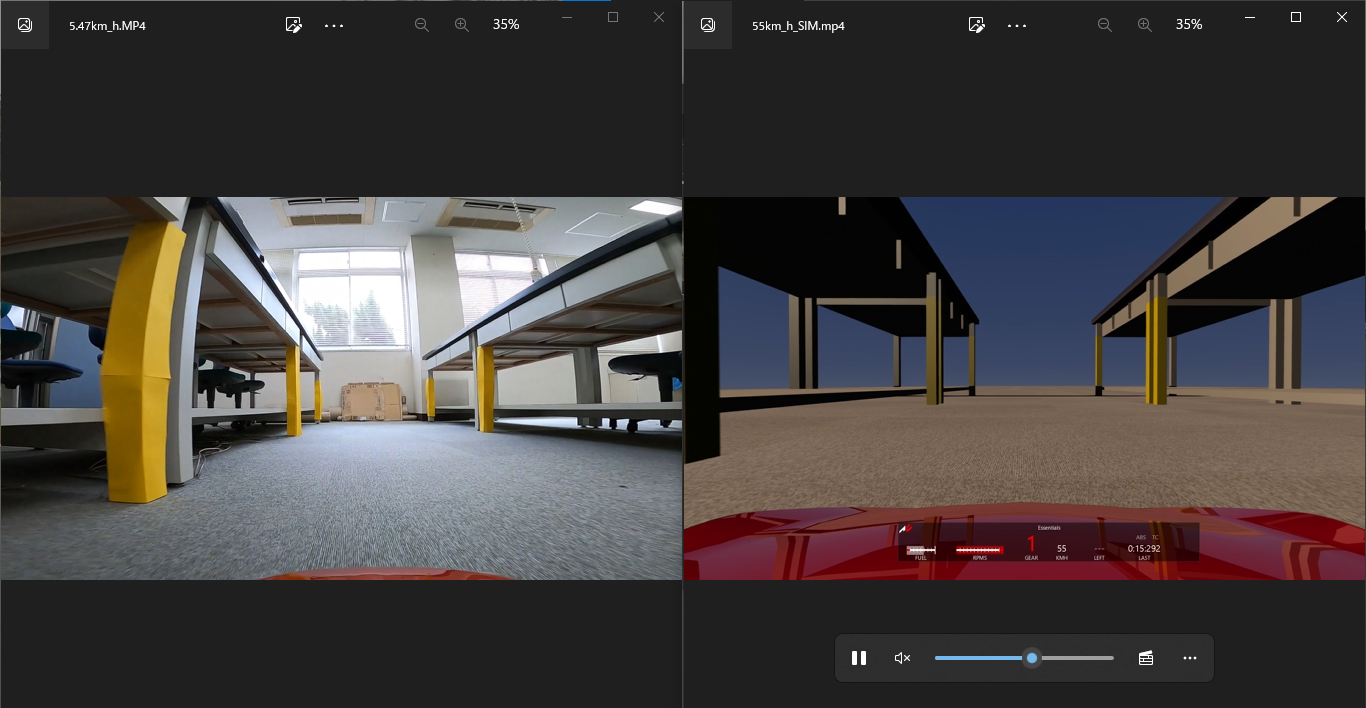
\includegraphics[width=\linewidth]{img/10.png}
  \caption{実験の様子}
  \label{taikan:hikaku}
  \end{center}
\end{figure}

\clearpage
\subsubsection{実験結果}
実測値とスケールスピードの計算結果を表\ref{taikan:table1}に示す。RCカーのスピードはモータの回転数を回転数計で計測し、
計算を行って、時速への変換を行っている。なお、モータの回転数は10回計測した際の平均値を採用している。
 
\begin{table}[ht]
\centering
\caption{実速度とスケールスピードの計算結果}
\scalebox{.83}{
\begin{tabular}[t]{rrrrrr}
\toprule
パルス入力値\si{[\micro s]}&パルス測定値\si{[\micro s]}&パルス誤差&回転数\si{[rpm]}&実速度\si{[km/h]}&スケールスピード\si{[km/h]}\\
\midrule
1348&1329&19&2194&24.81&78.47\\
1402&1386&16&1896&21.44&67.81\\
1438&1418&20&1589&17.97&56.83\\
1458&1440&18&1337&15.12&47.82\\
1480&1460&20&1161&13.13&41.52\\
1502&1482&20&854.6&9.666&30.57\\
\bottomrule
\label{taikan:table1}
\end{tabular}}
\end{table}%

モータの回転数を時速に変換する式を式\eqref{taikan:eq:motor}に示す。
\begin{align}
  v_{km} = d \times r \times 0.01885 \label{taikan:eq:motor}
\end{align}
ここで、$v_{km}$:時速、$d$:ホイールの直径\verb|(|6 \si{[cm]}\verb|)|、$r$:回転数\si{[rpm]}、\\0.001885:係数成分:$\frac{3600}{1000}\times\frac{2\pi}{60\times100}$
である。

RCカーのスケールスピード32 \si{[km/h]}\verb|(|実際の速度は10 \si{[km]}\verb|)|とDS上の速度32 \si{[km/h]}で比較した場合は、体感速度が一致しなかった。RCカーの速度10 \si{[km/h]}とDS上の速度100 \si{[km/h]}を比較した場合は、体感速度が一致した。
実験結果より、RCカーの操作視点カメラ映像の方が、DSの操作映像よりも体感速度が速いと評価されるため、RCカーのスケールスピードは体感速度と一致しないことを確認した。また、スケール比で走行させた場合に体感速度が一致したことから、
RCカーと自動車における移動ピクセル比は、スケール比の平方根ではなく、スケール比と同じ値をとることが検証された。
つまり、体感速度は、スケールスピードによる力学的相似ではなく、単純なスケール比を一致させた場合に一致すると言える。
次に、スケールスピードと体感速度が一致しない原因として検討したパラメータを挙げる。

\begin{enumerate}
  \item 映像中の風景線が流れるスピード\verb|(映像ピクセルの移動速度)|\\
  撮影範囲の道路における白線や、壁面と空との境界線等の風景線が単位当たりに移動する映像上でのピクセル数に注目することで、体感速度が異なることを確認した。
  \item 地上高\\
  RCカーの方が、実車と比べて操作視点の地上高が低いため、近くを見るようになる。景色は遠くより近くの方が速く流れるため、体感速度が上がる。これは、電車に乗って外を見ると、近くの建物は速く動くが、
  遠くの山などは遅く動くことと同じ現象である。RCカーの操作視点カメラの取り付け位置を変更し、変更前の走行映像と比較したが、体感速度に変化は見られなかった。
  \item 水平線に対する地面の割合\\
  地上高が低くなり、近くを見るようになることで、水平視点に対して、地面が見える割合が増えることによって体感速度が上がると推測した。水平線に対する地面の割合を変えるために、カメラの下半分を段ボールで隠し、
  水平線以上の景色のみしか撮影できないようにすることで、早く流れる近くの景色を遮断し、遠くの景色のみを写す。これによって体感速度を変化させる効果は得られなかった。
  \item 操作映像のクロップ・カメラの画角\\
  RCカーの操作視点カメラ映像を拡大クロップすることで、RCカーの体感速度が減少し、DSの映像とおおよそ一致したことを確認した。カメラ映像の画角体感速度の抑制に最も大きな効果を与えた。また、映像のクロップは、カメラ映像の画角を狭くする\verb|(|カメラの種類を広角・狭角と変更する\verb|)|ことと同じ効果を得ることができた。
\end{enumerate}

\subsection{体感速度のパラメータの選定}
前で述べた体感速度のパラメータのなかで影響度が高いものを選定する。映像のクロップ率を変化させることで、他の全てのパラメータが変化し、体感速度の中で最も影響の高いパラメータであることが明らかになった。

\subsection{映像のクロップによって体感速度変化を促す方法}
本実験で使用したカメラは水平視野角が120度である広角レンズを使用している。
このため、体感速度が実際よりも早く感じることがあった。カメラの種類\verb|(狭角・広角)|を変えることは容易ではないが、
撮影映像を編集することで体感速度を変化させる方法について検討した。その結果、映像をクロップ\verb|(映像の一部を拡大表示)|して画面全体に表示させることで、
元の映像よりも体感速度を減少させる効果を得た。

\subsubsection{映像のクロップ手法}
図\ref{taikan:crop1}、\ref{taikan:crop2}に映像クロップの概要を示す。以下にクロップの手順を示す。
\begin{enumerate}
  \item FPV映像をクロップし、元の解像度の比となるように拡大する。
  \item 拡大クロップしたRCカーの車体が見える部分\verb|(下部)|を削除する。
  \item 拡大クロップした映像の上部1を、DSの映像における水平消失点の流れと合わせるように切り取る。
  \item 拡大クロップした映像の残った部分を削除し、流れを合わせるように切り取った上部映像を、下部と繋がるように位置を下げる。
  \item 1の上部と連続している映像2を下のFPV映像から切り取る。
  \item 1の上部に2を繋ぎ合わせる。
\end{enumerate}

\begin{figure}[h]
  \begin{center}
  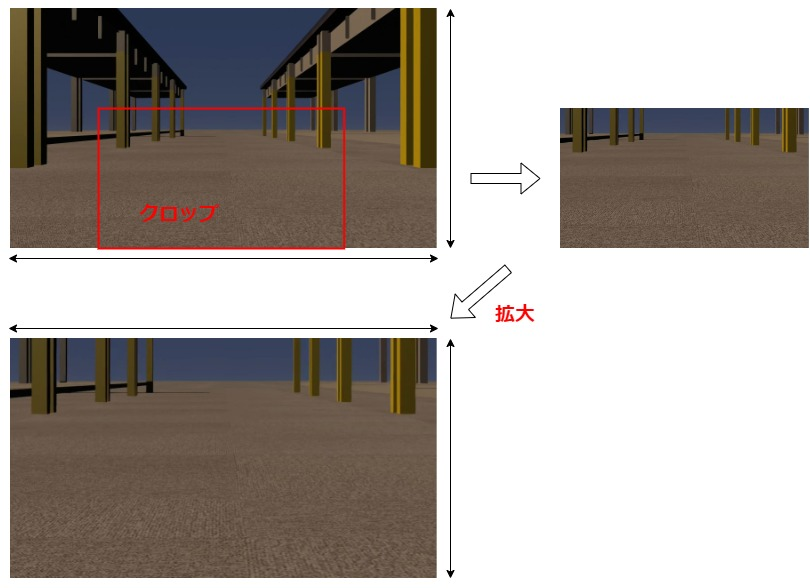
\includegraphics[width=.8\linewidth]{img/8_1.jpg}
  \caption{クロップ手順1}
  \label{taikan:crop1}
  \end{center}
\end{figure}

\begin{figure}[h]
  \begin{center}
  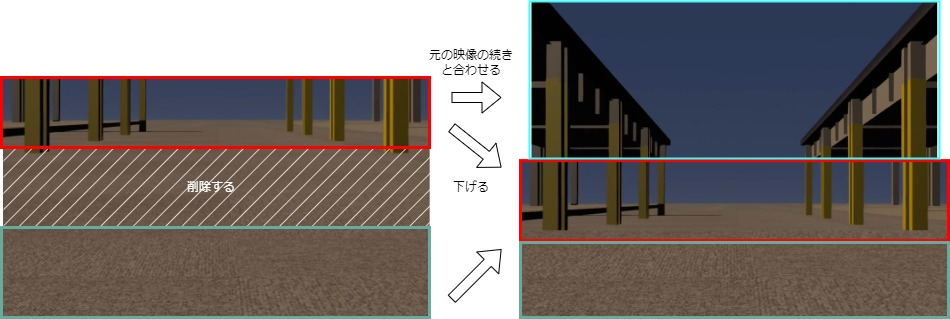
\includegraphics[width=.9\linewidth]{img/8_2.jpg}
  \caption{クロップ手順2}
  \label{taikan:crop2}
  \end{center}
\end{figure}
\clearpage
この実験によって、変化したパラメータについて述べる。クロップ率を増加させることで、映像の縦横の長さが減少し、視野角が減少することが明らかになった。
また、そのほかのパラメータも同時に変化し、クロップ率・視野角が体感速度の変化を制御するパラメータであることを定性的に示した。この時点では定量的な解析はできない。

\subsection{映像クロップによる体感速度の変化の仮説}
クロップ率の変化によって、体感速度が補正される根拠を以下に示す。
\begin{enumerate}
  \item 地上高\\
  手元の景色を排除し、遠くの景色を拡大したため、遠くの景色の流れが遅くなることから、体感速度が遅くなる。
  \item ピクセル\\
  映像のクロップにより、近くに見える映像がより遠い位置になるため、水平面より下の景色の流れが遅くなることで、ピクセルの移動速度が遅くなり、体感速度が遅くなる。
  \item 水平面より下の景色\\
  図\ref{taikan:cropzengo}にクロップ前後の見え方の変化について示す。

  \begin{figure}[h]
    \begin{center}
    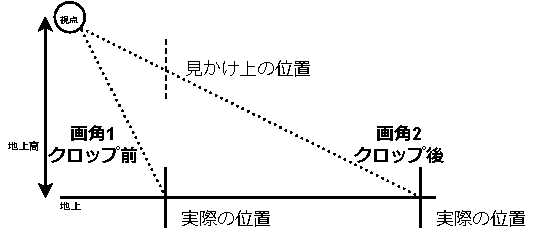
\includegraphics[width=.8\linewidth]{img/9_1.pdf}
    \caption{クロップ前後の見え方の変化}
    \label{taikan:cropzengo}
    \end{center}
  \end{figure}
  映像のクロップにより、クロップ前に見えていたものが前進する。それにより、見かけ上の位置がクロップ前と比べて、近くに見える映像がより遠い位置になるため、水平面よりも下の景色の見え始めが遠くなる。
よって、水平面より下の景色の流れが遅くなることで、体感速度が遅くなる。
\end{enumerate}

本研究以外にも同様の報告として、論文によると、映像のクロップによる体感速度の増強効果が、報告されている。
また、レース用ゲーム等で用いられる手法として取り入れられていることを確認している。

\clearpage

\subsection{体感速度のパラメータの導入}
体感速度変化で最も影響力のあるパラメータが映像のクロップとカメラの画角であることが分かった。
一般的に、走行映像を投影するカメラの画角に加えて、車両のドライバの視野角の変化が体感速度変化に寄与すると考えられている。
また、映像のクロップによってカメラの画角の変化が可能であることが共通の見識として共有されている。
つまり、映像のクロップによって、容易に車両中のドライバの視点の視野角を変化させることができ、体感速度を変化させることができる。
しかし、映像のクロップでは、ドライバの視野角を縮小する場合のみでしか検証ができない。
DSの視野角変更機能を用いることで、カメラの画角・ドライバの視野角を拡大する場合の検証を行うことができる。
そこで、本研究では、画角(視野角)・クロップというパラメータを導入し、映像のクロップを拡張し、
ドライバの視野角の拡大における体感速度の変化に関しても検討を行う。

